% Standalone source for the sliding-window QRC protocol figure.
% Build: pdflatex qrc_protocol.tex && pdftoppm -png -r 300 -singlefile qrc_protocol.pdf qrc_protocol
\documentclass[tikz, border=6pt]{standalone}
\usepackage{amsmath, amssymb}
\usetikzlibrary{decorations.pathreplacing}
\begin{document}
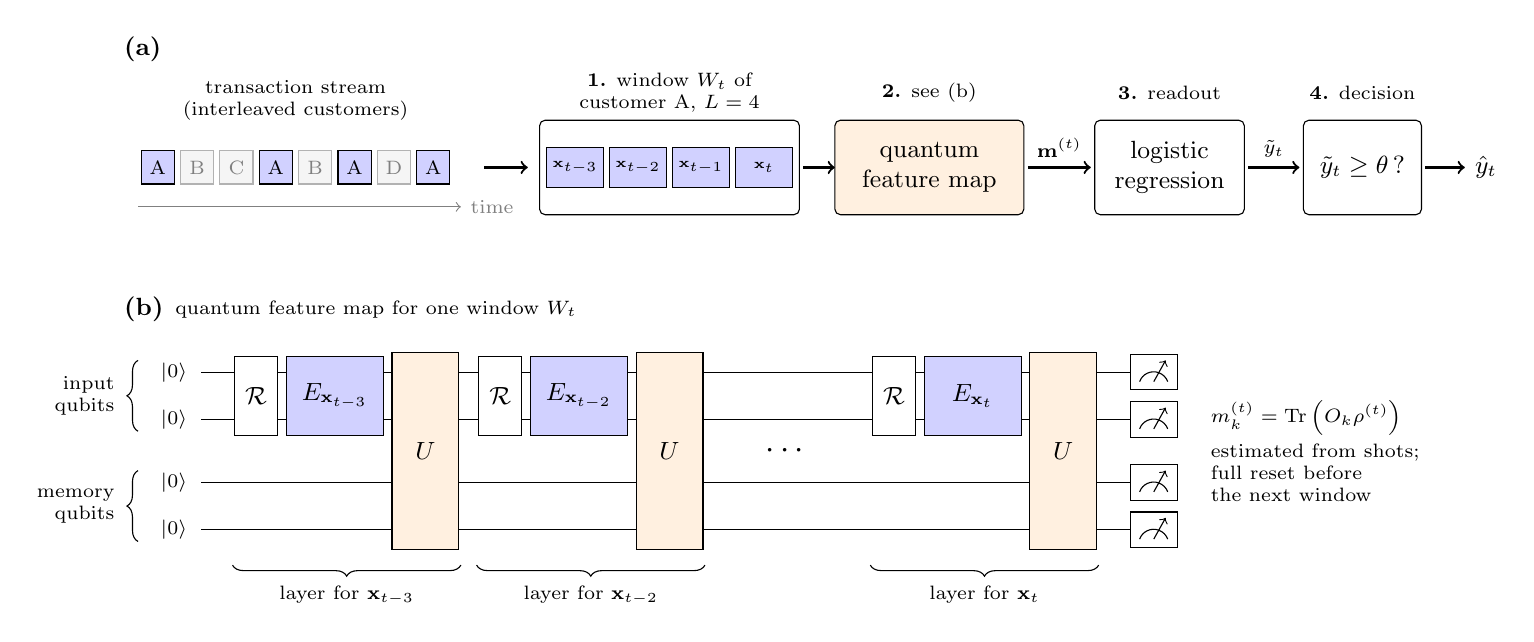
\begin{tikzpicture}[
    font=\small,
    box/.style={draw, rounded corners=2pt, align=center, minimum height=1.2cm, inner sep=3pt},
    arr/.style={->, thick},
    tx/.style={draw, minimum width=0.42cm, minimum height=0.42cm, inner sep=0pt, font=\scriptsize},
    cust/.style={tx, fill=blue!18},
    other/.style={tx, fill=gray!8, draw=gray!60, text=gray},
]
% ------------------------------------------------------------------ (a)
\node[anchor=west, font=\small\bfseries] at (-0.3, 2.1) {(a)};

% transaction stream, interleaved customers; customer A highlighted
\foreach \i/\c/\s in {0/A/cust, 1/B/other, 2/C/other, 3/A/cust, 4/B/other, 5/A/cust, 6/D/other, 7/A/cust} {
    \node[\s] at (0.25 + 0.5*\i, 0.6) {\c};
}
\node[font=\scriptsize, align=center] at (2.0, 1.45) {transaction stream\\(interleaved customers)};
\draw[->, gray] (0.0, 0.1) -- (4.1, 0.1) node[right, font=\scriptsize] {time};

\draw[arr] (4.4, 0.6) -- (4.95, 0.6);

% 1. windowing
\node[box, minimum width=3.3cm] (win) at (6.75, 0.6) {};
\foreach \i/\lab in {0/{-3}, 1/{-2}, 2/{-1}, 3/{}} {
    \node[cust, font=\tiny, minimum width=0.72cm, minimum height=0.5cm] at (5.55 + 0.8*\i, 0.6) {$\mathbf{x}_{t\lab}$};
}
\node[font=\scriptsize, align=center] at (6.75, 1.55) {\textbf{1.} window $W_t$ of\\customer A, $L=4$};

\draw[arr] (8.45, 0.6) -- (8.85, 0.6);

% 2. quantum feature map
\node[box, minimum width=2.4cm, fill=orange!12] (qfm) at (10.05, 0.6) {quantum\\feature map};
\node[font=\scriptsize] at (10.05, 1.55) {\textbf{2.} see (b)};

\draw[arr] (11.3, 0.6) -- node[above, font=\scriptsize] {$\mathbf{m}^{(t)}$} (12.1, 0.6);

% 3. readout
\node[box, minimum width=1.9cm] (ro) at (13.1, 0.6) {logistic\\regression};
\node[font=\scriptsize] at (13.1, 1.55) {\textbf{3.} readout};

\draw[arr] (14.1, 0.6) -- node[above, font=\scriptsize] {$\tilde{y}_t$} (14.75, 0.6);

% 4. decision
\node[box, minimum width=1.5cm] (dec) at (15.55, 0.6) {$\tilde{y}_t \geq \theta$\,?};
\node[font=\scriptsize] at (15.55, 1.55) {\textbf{4.} decision};
\draw[arr] (16.35, 0.6) -- (16.85, 0.6) node[right] {$\hat{y}_t$};

% ------------------------------------------------------------------ (b)
\begin{scope}[yshift=-1.4cm]
\node[anchor=west, font=\small\bfseries] at (-0.3, 0.2) {(b)};
\node[anchor=west, font=\scriptsize] at (0.35, 0.2) {quantum feature map for one window $W_t$};

% qubit wires: two input (top), two memory (bottom)
\foreach \y/\lab in {-0.6/in, -1.2/in, -2.0/mem, -2.6/mem} {
    \node[anchor=east, font=\scriptsize] at (0.75, \y) {$|0\rangle$};
    \draw (0.8, \y) -- (12.6, \y);
}
\draw[decorate, decoration={brace, amplitude=4pt}] (0.0, -1.35) -- (0.0, -0.45)
    node[midway, left=5pt, font=\scriptsize, align=right] {input\\qubits};
\draw[decorate, decoration={brace, amplitude=4pt}] (0.0, -2.75) -- (0.0, -1.85)
    node[midway, left=5pt, font=\scriptsize, align=right] {memory\\qubits};

% one layer: [R] [E_x] [U], starting at x-coordinate #1, input label #2
\newcommand{\protolayer}[2]{%
    \node[draw, fill=white, minimum width=0.55cm, minimum height=1.0cm] at (#1, -0.9) {$\mathcal{R}$};
    \node[draw, fill=blue!18, text width=1.0cm, align=center, minimum height=1.0cm] at (#1 + 1.0, -0.9) {$E_{\mathbf{x}_{#2}}$};
    \node[draw, fill=orange!12, minimum width=0.85cm, minimum height=2.5cm] at (#1 + 2.15, -1.6) {$U$};
    \draw[decorate, decoration={brace, mirror, amplitude=4pt}] (#1 - 0.3, -3.05) -- (#1 + 2.6, -3.05)
        node[midway, below=4pt, font=\scriptsize] {layer for $\mathbf{x}_{#2}$};
}
\protolayer{1.5}{t-3}
\protolayer{4.6}{t-2}
\node[fill=white, font=\large] at (8.25, -1.6) {$\cdots$};
\protolayer{9.6}{t}

% measurement
\foreach \y in {-0.6, -1.2, -2.0, -2.6} {
    \node[draw, fill=white, minimum width=0.6cm, minimum height=0.45cm] (m) at (12.9, \y) {};
    \draw (12.72, \y - 0.12) arc (160:20:0.19);
    \draw[->] (12.9, \y - 0.12) -- (13.05, \y + 0.15);
}
\node[font=\scriptsize, align=left, anchor=west] at (13.5, -1.6)
    {$m^{(t)}_k = \mathrm{Tr}\left(O_k \rho^{(t)}\right)$\\[2pt]estimated from shots;\\full reset before\\the next window};
\end{scope}
\end{tikzpicture}
\end{document}
